\documentclass{standalone}
\usepackage{tikz}
\begin{document}
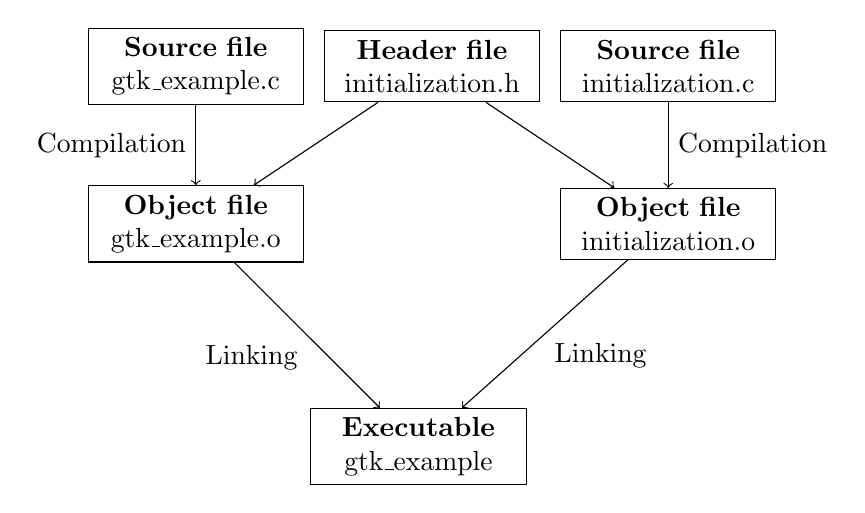
\begin{tikzpicture}[
    file/.style={draw,text width=2.5cm,align=center},
    arrow/.style={->,auto},
    node distance=2cm
  ]
  \node [file] (H) {\textbf{Header file}\\initialization.h};
  \node [file,left of=H,node distance=3cm] (A) {\textbf{Source file}\\gtk\_example.c};
  \node [file,right of=H,node distance=3cm] (B) {\textbf{Source file}\\initialization.c};
  \node [file,below of=A] (Ao) {\textbf{Object file}\\gtk\_example.o};
  \node [file,below of=B] (Bo) {\textbf{Object file}\\initialization.o};
  \node [file,below right of=Ao,node distance=4cm] (C) {\textbf{Executable}\\gtk\_example};
  \draw [arrow,auto=right] (A) -- node {Compilation} (Ao);
  \draw [arrow] (B) -- node {Compilation} (Bo);
  \draw [arrow] (H) -- (Ao);
  \draw [arrow] (H) -- (Bo);
  \draw [arrow,auto=right] (Ao) -- node {Linking} (C);
  \draw [arrow] (Bo) -- node {Linking} (C);
\end{tikzpicture}
\end{document}
